\begin{comment}
\documentclass[10pt]{article}
\usepackage{fullpage, graphicx, url}
\setlength{\parskip}{1ex}
\setlength{\parindent}{0ex}
\title{FLsetTextType}
\begin{document}


\begin{tabular}{ccc}
The Alternative Csound Reference Manual & & \\
Previous & &Next

\end{tabular}

%\hline 
\end{comment}
\section{FLsetTextType}
FLsetTextType�--� Sets some font attributes of the text label of a FLTK widget. \subsection*{Description}


 \emph{FLsetTextType}
 sets some attributes related to the fonts of the text label of the target widget. 
\subsection*{Syntax}


 \textbf{FLsetTextType}
 itype, ihandle
\subsection*{Initialization}


 \emph{itype}
 -- an integer number that modify the appearance of the target widget. 


  The legal values of \emph{itype}
 are: 


 
\begin{itemize}
\item 

 0 - normal label

\item 

 1 - no label (hides the text)

\item 

 2 - symbol label (see below)

\item 

 3 - shadow label

\item 

 4 - engraved label

\item 

 5- embossed label

\item 

 6- bitmap label (not implemented yet)

\item 

 7- pixmap label (not implemented yet)

\item 

 8- image label (not implemented yet)

\item 

 9- multi label (not implemented yet)

\item 

 10- free-type label (not implemented yet)


\end{itemize}
 When using \emph{itype}
=3 (symbol label), it is possible to assign a graphical symbol instead of the text label of the target widget. In this case, the string of the target label must always start with ``@''. If it starts with something else (or the symbol is not found), the label is drawn normally. The following symbols are supported: 

 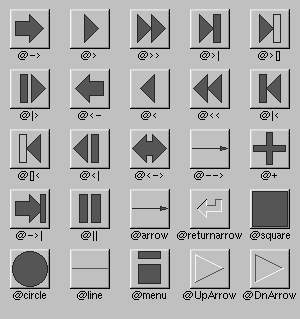
\includegraphics[scale=1]{symbols} 


 FLTK label supported symbols.


  The @ sign may be followed by the following optional ``formatting'' characters, in this order: 


 
\begin{enumerate}
\item 

 ``\#'' forces square scaling rather than distortion to the widget's shape.

\item 

 +[1-9] or -[1-9] tweaks the scaling a little bigger or smaller.

\item 

 [1-9] rotates by a multiple of 45 degrees. ``6'' does nothing, the others point in the direction of that key on a numeric keypad.


\end{enumerate}


  Notice that with \emph{FLbox}
 and \emph{FLbutton}
, it is not necessary to call \emph{FLsetTextType}
 opcode at all in order to use a symbol. In this case, it is sufficient to set a label starting with ``@'' followed by the proper formatting string. 


 \emph{ihandle}
 -- an integer number (used as unique identifier) taken from the output of a previously located widget opcode (which corresponds to the target widget). It is used to unequivocally identify the widget when modifying its appearance with this class of opcodes. The user must not set the \emph{ihandle}
 value directly, otherwise a Csound crash will occur. 
\subsection*{See Also}


 \emph{FLcolor}
, \emph{FLcolor2}
, \emph{FLhide}
, \emph{FLlabel}
, \emph{FLsetAlign}
, \emph{FLsetBox}
, \emph{FLsetColor}
, \emph{FLsetColor2}
, \emph{FLsetFont}
, \emph{FLsetPosition}
, \emph{FLsetSize}
, \emph{FLsetText}
, \emph{FLsetTextColor}
, \emph{FLsetTextSize}
, \emph{FLsetVal\_i}
, \emph{FLsetVal}
, \emph{FLshow}

\subsection*{Credits}


 Author: Gabriel Maldonado


 New in version 4.22
%\hline 


\begin{comment}
\begin{tabular}{lcr}
Previous &Home &Next \\
FLsetTextSize &Up &FLsetVal\_i

\end{tabular}


\end{document}
\end{comment}
